\documentclass{config/apuntes}

\title{Filogenia molecular}
\author{Sandra Mingo Ramírez}
\date{2024/25}
\acronym{PHYLO}

\usepackage[all]{nowidow}
\usepackage{listing}
\usepackage{color}
\usepackage{tabularx}

\definecolor{dkgreen}{rgb}{0,0.6,0}
\definecolor{gray}{rgb}{0.5,0.5,0.5}
\definecolor{mauve}{rgb}{0.58,0,0.82}

\lstset{frame=tb,
  language=Python,
  aboveskip=3mm,
  belowskip=3mm,
  showstringspaces=false,
  columns=flexible,
  basicstyle={\small\ttfamily},
  numbers=none,
  numberstyle=\tiny\color{gray},
  keywordstyle=\color{blue},
  commentstyle=\color{dkgreen},
  stringstyle=\color{mauve},
  breaklines=true,
  breakatwhitespace=true,
  tabsize=3
}

\begin{document}

\begin{abstract}
La filogenia molecular es la rama de la filogenia que analiza las diferencias moleculares hereditarias en las secuencias de ADN, ARN y proteínas para obtener información sobre las relaciones evolutivas de un organismo. El resultado de un análisis filogenético molecular se expresa en un árbol filogenético.
\end{abstract}

\pagestyle{plain}

\maketitle

\tableofcontents

%Examen de teoría 33% (algunas tipo test y otras de respuesta corta de conceptos), trabajo final 66%
%Para aprobar la asignatura es obligatorio obtener una nota mayor o igual a 5 puntos tanto en la parte de teoría como en el trabajo final.

%09/09 - Patricia Álvarez
\chapter{Introducción a la filogenia: principios y conceptos}
La filogenia es la determinación de la historia evolutiva de los organismos. Así, la filogenética es el estudio de: (i) la filogenia mediante el uso de árboles filogenéticos de los distintos organismos y (ii) las relaciones entre ellos. Ha habido varias iniciativas a lo largo de la historia (como \href{http://tolweb.org}{ToL Web}) que han intentado lograr crear árboles de todas las especies, cuyo número se estima por lo bajo que ronda los 3-5 millones. Estas estimaciones sobre la biodiversidad se realizan a partir de el número de grupos clave como los escarabajos, que son el grupo con mayor número de spp., en un lugar.

La filogenia es una disciplina muy consolidada; desde sus inicios, hace aproximadamente 200 años, sus representaciones no han cambiado mucho. La filogenia trabaja con árboles evolutivos, que son las \textbf{representaciones gráficas (patrones) de las relaciones ancestro-descendientes (relaciones históricas de parentescos) entre elementos}, que pueden ser especies, secuencias de genes, etc. Entender este patrón es esencial para realizar estudios comparativos de cualquier tipo, porque existen\textbf{ dependencias estadísticas entre los elementos que comparten ancestros comunes}. Conforme pasa el tiempo, se van aplicando diferentes y nuevos modelos evolutivos y se van depurando. En ultima instancia, se obtiene una mejor aproximación cuantos más datos se añadan (tanto más especies como más secuencias) a los modelos.

La filogenia sirve, entre otros, para: 
\begin{itemize}
\item Evolución de los seres vivos
\item Genómica: se puede observar mucho más allá y establecer límites entre especies. (Ej.: la evaluación es críptica. Si nos imaginamos a unos extraterrestres, no sabrán si clasificarnos a todos los humanos como una misma especie o distintas.)
\item Ingeniería genética
\item Farmacia
\item Epidemiología: ébola, VIH-1, etc. (Ver siguiente párrafo)
\item Biología de la conservación: discernir entre poblaciones y especies importa en relación con la clasificación de los espacios protegidos.
\item Control de plagas
\item Lingüística
\end{itemize}

La filogenética puede ser estudiada de diversas maneras. A menudo ha sido estudiada utilizando \textbf{registros fósiles}, que contienen información sobre la morfología de los antepasados de las especies actuales y la cronología de sus divergencias. Esto permite datar las filogenias. Sin embargo, el uso de registros fósiles presenta muchas limitaciones: pueden estar disponibles sólo para determinadas especies, los datos existentes de fósiles pueden estar fragmentados, la recolección de datos está limitada por la abundancia, hábitat, rango geográfico y otros factores; y las descripciones de los rasgos morfológicos son a menudo ambiguas (múltiples factores genéticos). Por todo esto, utilizar registros fósiles para determinar relaciones filogenéticas puede producir \textbf{sesgos}. Además, los fósiles de microorganismos son prácticamente inexistentes imposibilitando el uso de este enfoque. Afortunadamente, los \textbf{datos moleculares} que están en la forma de secuencias de ADN o de proteínas pueden ser también muy útiles para proporcionar una perspectiva de la evolución de los organismos, como el ARN 16S. Debido a que los genes son el medio para registrar las mutaciones acumuladas, éstos pueden servir como "fósiles moleculares". A través del análisis comparativo de secuencias de ADN de una serie de organismos relacionados, la historia evolutiva de los genes e incluso de los organismos puede ser revelada. La ventaja de utilización de datos moleculares es que son más numerosos que los registros fósiles y más fáciles de obtener. Además, no hay ningún sesgo de muestreo, como el que hay en los registros fósiles reales. Por tanto, es posible construir árboles filogenéticos más precisos y robustos utilizando datos moleculares. Como ejemplos, la filogenética se ha usado para datar y ubicar el origen del ébola en el brote de 2014 o el paciente 0 del VIH-1 en 1970.

Las filogenias, al ser una reconstrucción de la evolución de los caracteres, se construyen a partir de un registro/evidencias indirecto/as del proceso evolutivo. Por tanto, se deben realizar test de homología comprobar que los caracteres son comparables entre sí al compartir un origen común (homologías) y discernirlas de las homoplasias. De esa forma se obtiene información para construir clasificaciones y hacer predicciones dentro de un marco temporal cuando es posible obtenerlo.

\section{Conceptos básicos}
Los árboles filogenéticos suelen ser binarios, estando compuestos por \textbf{nodos externos o terminales} y \textbf{nodos internos} unidos por \textbf{ramas} que parten de una \textbf{raíz}. A través de las diferentes ramas se van reconstruyendo las relaciones entre las especies. Los \textbf{nodos internos son hipótesis evolutivas de posibles ancestros comunes} de los cuales normalemente faltan datos para confirmar o descartar la teoría. En las distintas ramas se pueden representar la transformación de caracteres que aparecen a nivel genético y que se transmiten por herencia.  

\begin{figure}[htbp]
\centering
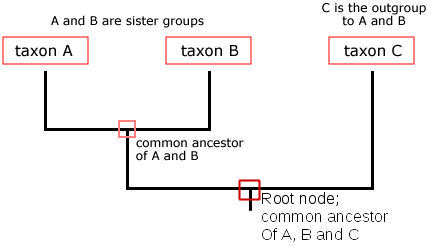
\includegraphics[width=0.5\linewidth]{figs/taxon-tree.png}
\caption{Partes de un árbol filogenético.}
\end{figure}

Se denominan \textbf{grupos hermanos} a los nodos terminales que parten de un mismo nodo interno, es decir, dos taxones que compartan un ancestro común no compartido por ningún otro taxón. El \textbf{grupo externo (outgroup)} es aquel que se encuentra más alejado y parte de una rama distinta desde la raíz. Normalmente, este outgroup se elige arbitrariamente para poder colocar la raíz donde se estima correcto. Todas las especies que se desarrollan desde una rama de la raíz se denomina \textbf{grupo interno o ingroup}. 

Los árboles filogenéticos se pueden representar sin enraizar o enraizado. Un árbol filogenético sin raíz no asume conocimiento de un ancestro común, solo posiciones de los taxones para mostrar sus relaciones relativas (no hay dirección de un camino evolutivo). Para describir la dirección de la evolución se necesita un árbol filogenético con raíz donde todas las secuencias bajo estudio tienen un ancestro o nodo raíz común (más informativo). Mientras que los árboles filogenéticos se centran en las relaciones evolutivas entre diferentes especies, las redes haplotípicas son representaciones gráficas sobre las relaciones evolutivas entre las diferentes poblaciones.

A la hora de visualización, hay varias formas de representar los árboles filogenéticos. Los distintos elementos no tienen un orden concreto; da igual si en un árbol los nodos terminales están en distinto orden mientras que las ramas sigan el mismo camino. En general, se suelen poner los nodos terminales de manera que sea más fácil de leer a simple vista.

\begin{figure}[htbp]
\centering
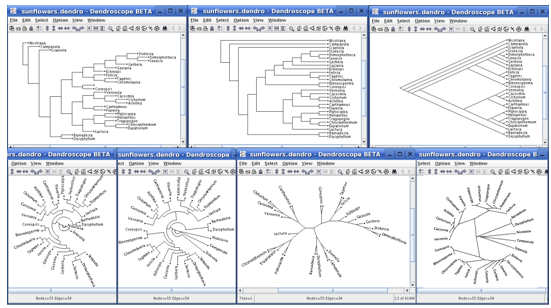
\includegraphics[width=0.5\linewidth]{figs/representaciones-arboles.png}
\caption{Distintas representaciones de los árboles filogenéticos.}
\end{figure}

\section{Politomías}
La topología es la forma en que se ramifica un árbol. Cuando todas las ramas se bifurcan en un árbol filogenético, éstas son denominadas como una \textbf{dicotomía}. Por el contrario, si de un nodo surgen más de dos ramas (descendientes), entonces se denomina \textbf{politomía}.

\begin{figure}[htbp]
\centering
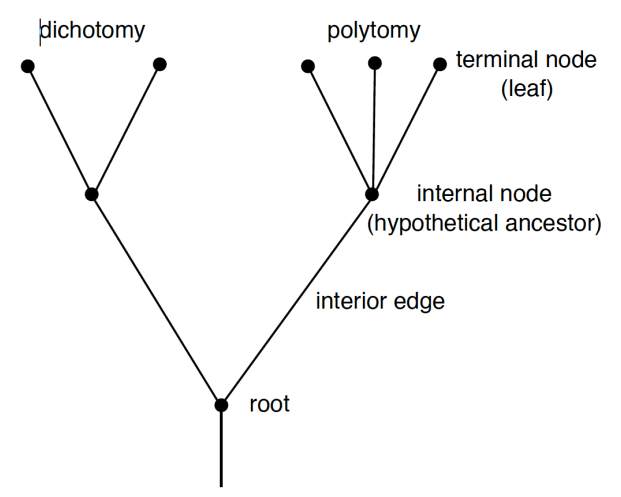
\includegraphics[width=0.3\linewidth]{figs/dichotomy-polytomy.png}
\caption{Diferencia entre dicotomía y politomía.}
\end{figure}

Los árboles filogenéticos se consideran resueltos cuando de un nodo interno salen las distintas terminales. En la mayoría de casos, los árboles son no resueltos y tienen politomías, es decir, que desde un nodo interno no se sabe cómo han avanzado las especies. A partir de ahí solo se pueden añadir más datos, pintar uniones con un bootstrap bajo (es decir, un bajo soporte de esa bifurcación), o justificar que estamos atestiguando un momento de especiación. Dentro de las hipótesis filogenéticas siempre hay más de una solución (se producen varios árboles igualmente óptimos), así que el árbol final se debe elegir. Un árbol de consenso puede ser construido mostrando las porciones de bifurcación resueltas comúnmente y colapsando aquellas que no concuerdan entre los árboles. En un árbol de consenso estricto, todos los nodos en conflicto son colapsados.

\begin{figure}[htbp]
\centering
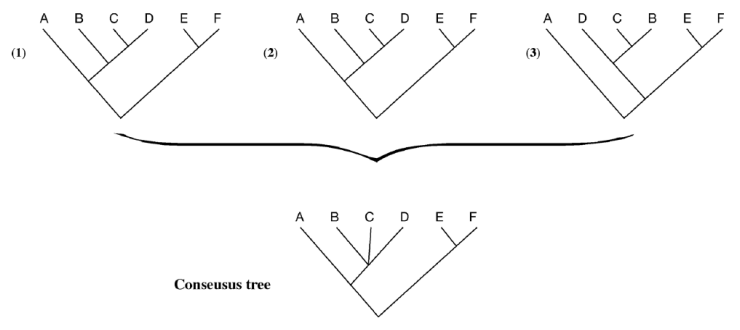
\includegraphics[width=0.5\linewidth]{figs/consensus-tree.png}
\caption{Árbol de consenso.}
\end{figure}

\section{Tipos de árboles filogenéticos}
Existen distintos tipos de árboles filogenéticos. Los \textbf{filogramas (phylogram}) miden en las ramas los cambios que ha habido por sitio, por lo que las longitudes de las ramas representan a escala la cantidad de divergencia evolutiva. Tienen la ventaja de mostrar tanto las relaciones evolutivas como la información sobre el tiempo relativo de divergencia de las ramas. Los \textbf{cladogramas (cladogram)} muestran la similitud de los distintos elementos, pero las longitudes de sus ramas no son proporcionales al número de cambios evolutivos y, por tanto, no tienen ningún significado filogenético. Los \textbf{cronogramas (chronogram)} representan la relación de los elementos de forma temporal.

\begin{table}[h]
\centering
\begin{tabular}{l c c}
\hline
\multicolumn{1}{l}{[phyl(o) gr. 'raza', 'estirpe']} & \multirow{3}{1em}{+} & \multirow{3}{12em}{[-gram-ma gr. 'representación gráfica']} \\
\multicolumn{1}{l}{[klad(o) gr. 'rama']} & & \\
\multicolumn{1}{l}{[khron(o) gr. 'tiempo']} & & \\
\hline
\end{tabular}
\caption{Tabla con términos griegos y sus significados.}
\end{table}

\begin{figure}[htbp]
\centering
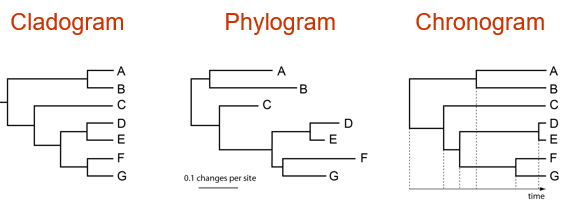
\includegraphics[width=0.5\linewidth]{figs/tipos-arboles.png}
\caption{Tipos de árboles filogenéticos.}
\end{figure}

\section{Inferencia filogenética}
Cualquier episodio histórico es, por definición, irrecuperable. La única forma que tenemos de reconstruirlo es a través del estudio de sus efectos. Por ello, la reconstrucción filogenética es un proceso de inferencia: se intenta obtener la mejor estimación posible de una historia evolutiva basada en la información incompleta y con frecuencia ruidosa contenida en los datos. Las evidencias que se emplean se basan en la morfología (comparación entre caracteres de especies), la ultraestructura (cortes vistos al microscopio electrónico), embriología (fases del desarrollo embrionario), la paleontología (registro fósil), la etología (comportamiento animal -> para estudiar evolución simpátrica), la bioquímica y las moléculas. 

Un \textbf{carácter} es una característica de los taxones que, en principio, es heredada (si no es heredada, no se puede utilizar la filogenia). El \textbf{estado de carácter} es el valor específico que toma un carácter en un taxón concreto. Por ejemplo, un carácter sería tener ojos y el estado de ese carácter sería 2 para humanos y 8 para algunas arañas.

\section{Homología}
La \textbf{homología} es la relación que existe entre dos partes orgánicas diferentes de dos organismos distintos cuando sus determinantes genéticos tienen el mismo origen evolutivo, es decir, cuando un mismo órgano tiene diversas formas y funciones. Los caracteres que se estudian en filogenia deben ser homólogos. Se compara la semejanza de una estructura debido a la herencia común. Por el contrario, la analogía es una estructura semejante a otra o que tiene la misma función, pero cuyo desarrollo embrionario y origen son diferentes. No se presentan en un antepasado común (como en el caso de los caracteres homólogos), si no que es fruto de convergencia evolutiva.

En genética y biología molecular, también existe homología en las secuencias. Se distinguen dos tipos: la ortología y la paralogía. Los \textbf{genes ortólogos} son semejantes por pertenecer a dos especies que tienen un antepasado común. Los \textbf{genes parálogos} son aquellos que se encuentran en el mismo organismo y cuya semejanza revela que uno procede de la duplicación del otro (y puede adquirir funciones diferentes del gen original). La ortología requiere que se haya producido especiación, mientras que esta no es necesaria en el caso de la paralogía, que puede producirse solo en los individuos de una misma especie. Por ello, idealmente se deben comparar caracteres ortólogos para hacer las reconstrucciones filogenéticas.

\begin{figure}[htbp]
\centering
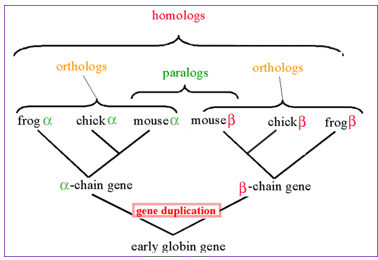
\includegraphics[width=0.5\linewidth]{figs/ortologos-paralogos.png}
\caption{Homología en genes de la hemoglobina.}
\end{figure}

%11/09 - Patricia Álvarez
\subsection{Tipos de homología}
En cladística, se emplean unas clasificaciones de las propiedades de organismos basándose en similitudes derivadas. Una \textbf{plesiomorfía} se refiere al estado \textit{ancestral} (o \textit{primitivo}) de un carácter que comparten distintas especies por heredarlo del antepasado común; en el árbol filogenético de ejemplo se presenta en los ancestros y los grupos externos. En contraposición, la \textbf{apomorfía} es un carácter novedoso evolutivamente y se dice que es \textit{derivado}, ya que deriva de otro rasgo perteneciente a un taxón ancestral filogenéticamente próximo. Así, se emplean los adjetivos plesiomófico y apomórfico en lugar de primitivo y avanzado para evitar juicios de valor sobre la evolución de los carácteres. 
Además, una \textbf{sinapomorfía} es una apomorfía (carácter exclusivo) compartida por un ancestro común y todos sus descendientes; y una \textbf{simplesiomorfía} se refiere a una plesiomorfía (carácter ancestral) compartida por dos o más taxa. Finalmente, una \textbf{autapomorfía} es un carácter novedoso y único de un taxón que no aparece en el antepasado, por lo que no lo comparte con ningún otro. 

\begin{table}[htbp]
\begin{mdframed}[backgroundcolor=black!10]
    \centering
    El prefijo "sin" viene de "compartido". Por tanto, los caracteres sinapomorfos son caracteres apomorfos compartidos, mientras que las simplesiomorfías son plesiomorfías compartidas.
    \end{mdframed}
\end{table}

\begin{table}[h]
\centering
\begin{tabular}{l c c }
\hline
\multicolumn{1}{l}{[sýn- gr. 'con', 'unión']} & \multirow{4}{*}{+} & \multirow{2}{*}{[morph gr. 'forma']} \\
\multicolumn{1}{l}{[plēsio- gr. 'cercano']} & &  \\
\multicolumn{1}{l}{[aut(o)- gr. 'que actúa por sí mismo']} & & \multirow{2}{*}{[-íā gr. 'cualidad']}  \\
\multicolumn{1}{l}{[apó- gr. 'a partir de' (derivado, novedoso)]} & & \\
\hline
\end{tabular}
\caption{Tabla con términos griegos y sus significados.}
\end{table}

\begin{figure}[htbp]
\centering
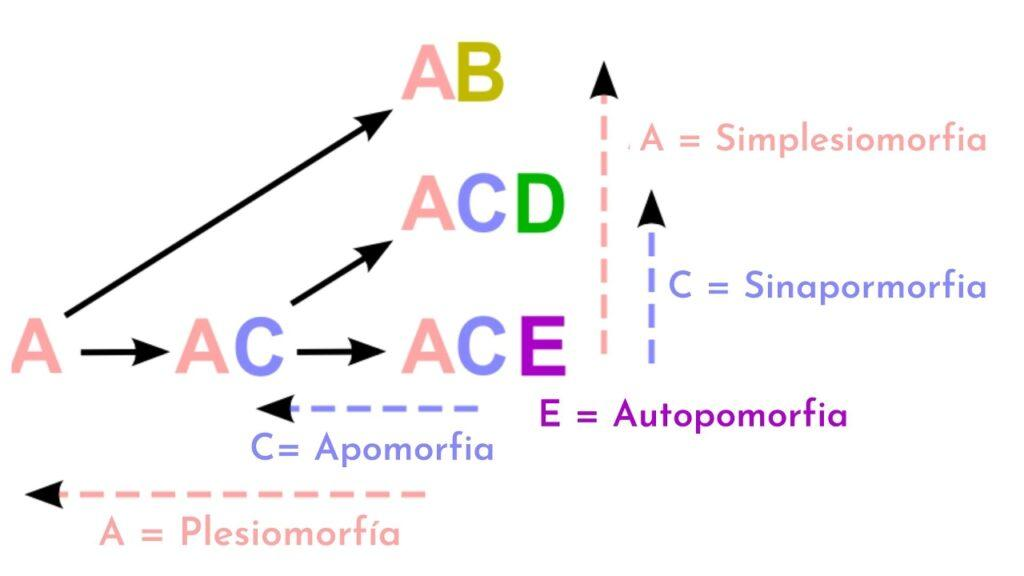
\includegraphics[width=0.5\linewidth]{figs/sinapomorfia.jpg}
\caption{Tipos de homología en el árbol filogenético (tumbado). El carácter A es plesiomórfico al estar en el ancestro. El carácter C es apomórfico al ser una novedad evolutiva. En los nodos terminales, el carácter A se considera simplesiomórfico al estar compartido por los descendientes y ser un carácter ancestral. Por el contrario, el carácter C en los nodos terminales es sinapomórfico por ser un carácter novedoso y estar compartido en el ancestro en el que surgió y sus descendientes. Los caracteres B, D y E son autopomorfos por estar presentes en un único nodo terminal.}
\end{figure}

\subsection{Homoplasia}
La homoplasia es el cambio evolutivo paralelo que hace que dos organismos presenten un mismo carácter adquirido independientemente. La \textbf{convergencia} se da cuando dos estructuras similares han evolucionado independientemente a partir de estructuras ancestrales distintas y por procesos de desarrollo diferentes. Se considera que el \textbf{paralelismo} involucra patrones de desarrollo similares en líneas evolutivas diferentes, pero próximas. La diferencia con la convergencia es que en el paralelismo, hay un ancestro que no presenta un carácter y dos descendientes directos sí presentan esa novedad evolutiva, mientras que en la convergencia los descendientes con carácter no tienen el mismo ancestro común directo. No obstante, en la práctica, la distinción entre convergencia y paralelismo es un tanto arbitraria porque no existe una regla exacta para limitar la antigüedad del antepasado común. Finalmente, en la \textbf{reversión}, un organismo adquiere un carácter de sus antepasados más lejanos. Esto implica que uno o más caracteres adquiridos previamente se han eliminado y se han vuelto a los más anteriores. 

\begin{figure}[htbp]
\centering
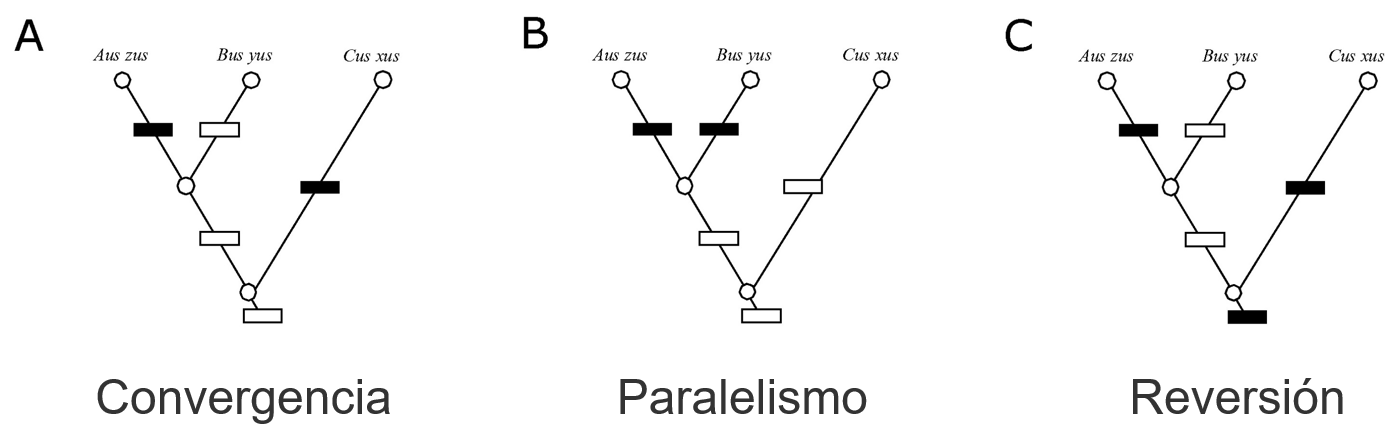
\includegraphics[width=0.5\linewidth]{figs/homoplasia.png}
\caption{Diferencias entre convergencia, paralelismo y reversión.}
\end{figure}

\subsection{Agrupamientos}
Un \textbf{grupo monofilético} es un clado que contiene un ancestro y todos sus descendientes, formando así un solo grupo evolutivo. Un \textbf{grupo parafilético} es similar, pero excluye a algunos de los descendientes que han sufrido cambios significativos. Un grupo con miembros de líneas evolutivas separadas se llama \textbf{polifilético}, conteniendo así grupos de especies con distintos ancestros comunes. 

\begin{figure}[htbp]
\centering
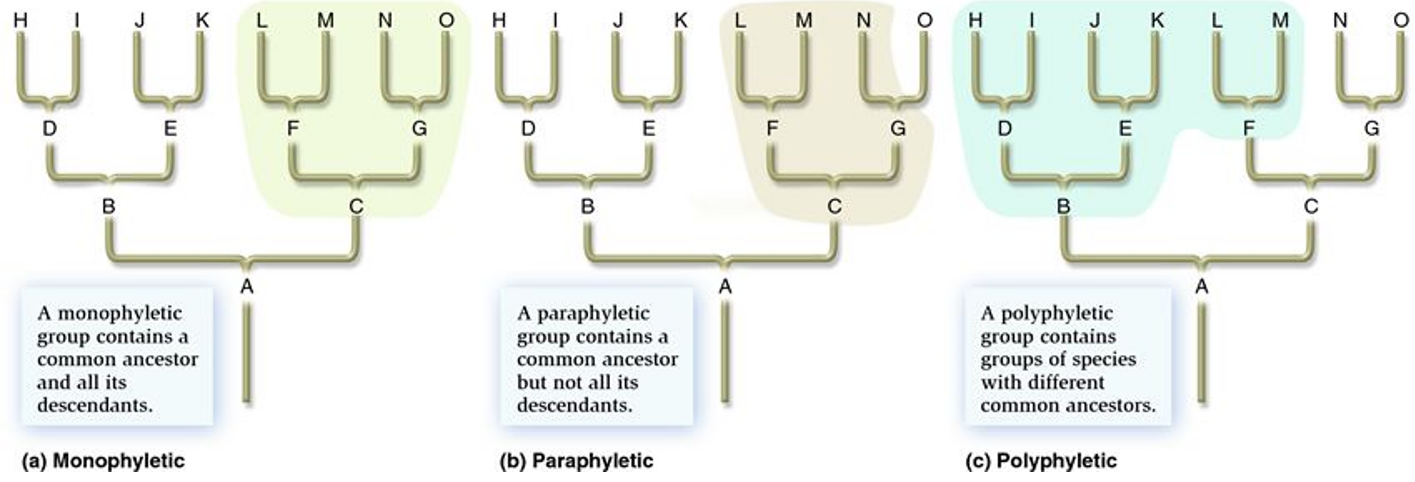
\includegraphics[width=0.5\linewidth]{figs/agrupamientos.png}
\caption{Agrupamientos de grupos monofiléticos, parafiléticos y polifiléticos.}
\end{figure}

De esa forma, los grupos monofiléticos presentan sinapomorfía, los grupos parafiléticos presentan simplesiomorfía, y los grupos polifiléticos homoplasia. 

\begin{figure}[htbp]
\centering
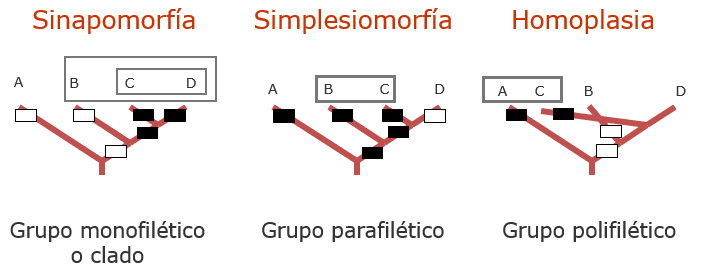
\includegraphics[width=0.5\linewidth]{figs/homoplasia-agrupamientos.png}
\caption{Grupos y caracteres que se apoyan.}
\end{figure}

\subsection{Fenotipo vs moléculas}
Tradicionalmente se han empleado los \textbf{carácteres fenotípicos} para establecer las relaciones filogenéticas. Esto se debe a que suelen ser carácteres evolutivamente relevantes y complejos menos proclives a la homoplasia. Además, son los únicos carácteres disponibles en algunos casos como en fósiles o especímenes raros. No obstante, puede haber problemas de codificación de taxones supraespecíficos como terminales (quimera ¿¿NO??) y se pueden dar casos de subjetividad en la codificación de carácteres. Además, hay un número limitado de carácteres fenotípicos y podemos encontrar taxones altamente autapomórficos. 

Recientemente se están empleando \textbf{carácteres moleculares} al ser estrictamente heredables y no haber ambigüedades en la codificación. Por ello, determinar el estado de los carácteres es trivial. Hay ciertas regularidades en la evolución de los carácteres moleculares, y éstos son robustos frente a la distancia evolutiva. También son muy abundantes y ofrecen información temporal. El problema de los carácteres moleculares es que son más proclives a la homoplasia al tener solo 4 nucleótidos y 20 aminoácidos. La evolución de estos carácteres es compleja. Además, los árboles de genes no siempre coinciden con los árboles de especies. La determinación de la homología puede ser difícil por duplicación o pérdida de genes y alineamientos. 

Se suelen utilizar multitud de genes separados y analizarlos de forma separada. El consenso de análisis separados es una estimación conservadora de la filogenia. Algunos métodos filogenéticos sólo se pueden aplicar a ciertos tipos de datos. A nivel de especies, la concatenación de genes diferentes puede ser inapropiada si se da transferencia horizontal de genes, hibridación, duplicación de genes o coalescencia más profunda que el tiempo de divergencia. El conflicto entre caracteres se resuelve teniendo en cuenta toda la evidencia disponible y realizando análisis combinados. Diferentes tipos de datos proporcionan información a diferentes niveles filogenéticos. La señal filogenética aumenta debido a la congruencia entre caracteres de diferentes conjuntos de datos. 

Es importante que el conjunto de datos sea lo más completo posible. Es necesario hacer un muestreo de taxones (incluyendo los grupos externos) y genes razonable y justificado. 

%11/09 - Patricia Álvarez
\chapter{Alineamiento de secuencias}
Decidir qué caracteres investigar, y cómo codificarlos, es un primer paso crucial en cualquier análisis filogenético. 

\section{Tipos de caracteres}
Hay \textbf{sitios invariables} que no cambian en los distintos taxones. También hay \textbf{sitios filogenéticamente neutrales} que son autapomorfías. Los \textbf{sitios filogenéticamente informativos} son comunes por pares, por lo que son sinapomorfías. 

\begin{figure}[htbp]
\centering
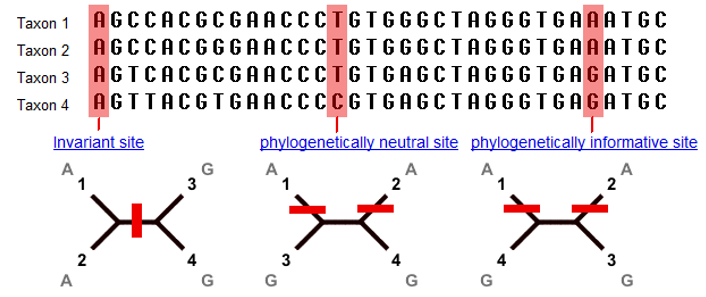
\includegraphics[width=0.5\linewidth]{figs/sitios-informativos.png}
\caption{Sitios en una secuencia invariantes (no cambian entre los distintos taxones), filogenéticamente neutrales (solo cambia en un taxón) y filogenéticamente informativos (permiten dicotomía).}
\end{figure}

Los caracteres pueden ser \textbf{binarios 0/1} (presentes o ausentes), \textbf{multiestado} o \textbf{binarios V/S} (transversiones o transiciones). Los caracteres también pueden ser \textbf{discretos o continuos}. La codificación de caracteres continuos no se pueden incluir fácilmente en las matrices de caracteres, por lo que se debe realizar una categorización arbitraria. Idealmente, se deben buscar divisiones naturales, es decir, estados discretos de un carácter de variación continua. 

\section{Ponderación de los caracteres}
Se puede emplear un valor relativo de los diferentes caracteres y transformaciones como indicadores de las relaciones filogenéticas entre taxones. Se puede realizar una ponderación uniforme, que minimiza los supuestos del análisis, o una ponderación diferencial, en la que no todas las características de un organismo tienen el mismo valor como evidencias filogenéticas. 

\subsection{Ponderación \textit{a priori}}
En la ponderación \textit{a priori} de caracteres morfológicos, los taxónomos pueden tener muchas razones para asumir que diferentes caracteres tienen diferente importancia filogenética. Pero eso tiene dos problemas: diferentes opiniones expertas y, en caso de acuerdo, el peso proporcional que se le da a cada carácter. Se introduce precisamente el tipo de subjetividad que el análisis cladístico pretende evitar.

\subsection{Ponderación \textit{a posteriori}}
El método más utilizado y aplicado, denominado \textbf{ponderación implícita}, se basa en Goloboff (1993): la primera vez que un carácter cambia de estado en un árbol, este cambio de estado recibe el peso «1»; los cambios posteriores son menos «costosos» y reciben pesos menores a medida que la tendencia de los caracteres a la homoplasia se hace más evidente. Los árboles que maximizan la función cóncava de homoplasia resuelven el conflicto de caracteres a favor de los caracteres que tienen más homología (menos homoplasia) e implican que el peso medio de los caracteres sea lo más alto posible.

Goloboff reconoce que los árboles con los pesos medios más elevados son los que más «respetan» los datos: un peso medio bajo implica que la mayoría de los caracteres están siendo «ignorados» por los algoritmos de construcción de árboles. Aunque originalmente se propuso con una ponderación severa de k=3, Goloboff prefiere ahora concavidades más «suaves» (por ejemplo, k = 12), que han demostrado ser más eficaces en casos simulados y del mundo real.

$$F = \sigma fi, fi = \frac{k}{k+(s-m)} $$

siendo m el número mínimo de pasos, s el número de pasos observados y k la constante de concavidad.

\subsection{Secuencias de ADN}
 Generalmente, se toma la tasa de sustitución como medida de la fiabilidad de la información filogenética del marcador. Se entiende entonces homoplasia como saturación. Las transversiones evolucionan lentamente y aumentan su frecuencia a medida que pasa el tiempo. Las transiciones se saturan a partir de cierta distancia filogenética, perdiéndose su señal. 
 
El coste de las transformaciones se determina empíricamente mediante matrices de costes (stepmatrices). 

\section{Polaridad de los caracteres}
Necesitamos conocer la polaridad de los caracteres para poder enraizar los árboles. Para ello, se debe establecer qué carácter es ancestral y qué carácter es derivado. Utilizando un \textbf{criterio ontogenético}, se ve cómo se forma el carácter durante el desarrollo para poder establecer la polaridad. En caso de que no quede claro tras ese criterio, se compara con el outgroup para establecer el estado primitivo del carácter. 

\section{Homología de los caracteres moleculares}
Cuando analizamos secuencias, asumimos que son de moléculas heredadas de ancestros a descendientes (ortólogos). Cada secuencia está formada por muchos caracteres (cada posición en la secuencia). Por ello, un primer paso es determinar el estado de cada uno de esos caracteres en cada taxón de la matriz. Importante: La homología de los caracteres moleculares, como la de cualquier otro tipo de carácter, es un concepto cualitativo. Las secuencias del gen A de dos taxones son homólogas, o bien no lo son. Igualmente, la posición X en la secuencia de un taxón es homóloga de la posición Y en la secuencia de otro taxón, o bien no lo es. Pero NO puede decirse que las secuencias de dos taxones muestren mayor o menor homología (por ejemplo, en \%). Podrán tener diferente porcentaje de similitud (p. ej., \% de bases o aminoácidos idénticos en posiciones homólogas), pero o son homólogas o no lo son.

\subsection{Aplicación del concepto de homología a los genes: alineamiento de secuencias}
Un alineamiento es una hipótesis acerca de la homología posicional de diferentes secuencias de bases o aminoácidos. El alineamiento tiene como objetivo identificar qué posiciones son homólogas en diferentes secuencias. Cada posición de la secuencia (residuo = nucleótido o aminoácido) se interpreta como un carácter que puede tomar diferentes valores (estados de carácter: una de 4 bases, o uno de 20 aminoácidos). El alineamiento asume parsimonia: el cambio evolutivo es improbable, de modo que los segmentos de secuencia coincidentes sirven de guía para identificar posiciones homólogas. Eventualmente se identifican cambios, que cuando son compartidos por varias especies son informativos para la reconstrucción de filogenias.

Las secuencias pueden no tener la misma longitud. Los gaps son marcadores de posición que introducimos en los alineamientos para mantener la homología posicional. Representan eventos de inserción o pérdida denominados indels (del inglés insertion/deletion). La ventaja es que los indels son, en principio, menos propensos a la homoplasia que las sustituciones de bases, muy utilizadas en análisis de parsimonia. No obstante, los indels son difícilmente gestionables por la mayoría de los modelos de evolución molecular. 

Es importante elegir un buen alineamiento, ya que la calidad del alineamiento influye en la calidad de la inferencia filogenética. 

%\subsection{Alineamientos globales vs locales} -> se lo saltó
%En el \textbf{alineamiento global}, se intenta alinear cada residuo en cada secuencia. Son especialmente útiles para alinear secuencias emparentadas de tamaño similar (las que se usan para la reconstrucción filogenética). El \textbf{alineamiento local} se utiliza para secuencias poco parecidas que se supone que contienen regiones similares, o para identificar la ubicación de motivos concretos en contextos más amplios (por ejemplo, BLAST). 

\subsection{Decidir el mejor alineamiento}
No existe ningún procedimiento automático para elegir objetivamente el mejor alineamiento: hay que valorar la calidad de los diferentes alineamientos posibles y elegir el que nos parezca mejor. Elegimos como mejor alineamiento el supuesto más razonable de acuerdo con un algoritmo informático y el ojo experimentado. En cualquier caso, es siempre importante examinar el resultado críticamente para valorar si tiene sentido desde un punto de vista biológico.

No todos los alineamientos son igualmente parsimoniosos. Para valorar la calidad de los alineamientos, se han propuesto diferentes mecanismos de puntuación. Se puede realizar una \textbf{puntuación por identidad}. Un alineamiento de dos secuencias puede interpretarse como una matriz con dos filas y n columnas (n = longitud del alineamiento). Las posiciones (columnas) con idéntico residuo (base o aminoácido) tienen una puntuación = 1. La puntuación del alineamiento es la suma de las puntuaciones de todas sus posiciones. El alineamiento óptimo es el que maximiza la identidad de las columnas. No obstante, los gaps no penalizan, por lo que pueden darse alineamientos con misma puntuación, pero más posiciones de diferencia. Por tanto, se pueden aplicar penalizaciones para los huecos en la secuencia, ya sea introduciendo penalizaciones por la apertura de los huecos o por la extensión de los huecos abiertos. Estos últimos son típicamente menores que las impuestas por apertura. Por ejemplo, se puede aplicar una penalización de -2 por apertura de gap y de -1 por extensión del gap abierto.  

\begin{figure}[htbp]
\centering
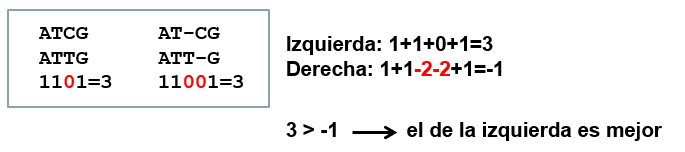
\includegraphics[width=0.5\linewidth]{figs/mejor-alineamiento.png}
\caption{Ejemplo de cálculo del mejor alineamiento.}
\end{figure}

No tiene mucho sentido alinear las secuencias de ADN de los genes codificantes de proteínas. Es mejor traducir las secuencias de ADN a secuencias de aminoácidos y alinear éstas últimas. Existen varios programas para alineamiento múltiple: clustal W/X/Omega, MAFFT, Muscle, T-Coffee, Dialign 2, etc. 

%Nos saltamos la diapositiva 42 y de la 44 a la última.



%11/09 - Patricia Álvarez
\chapter{Modelos de evolución}
Todos los métodos de inferencia y reconstrucción filogenética implican una serie de \textbf{supuestos}, aunque éstos no se hagan explícitos: \begin{itemize}
\item Todos los sitios o posiciones cambian independientemente. 
\item Las tasas de evolución son constantes a lo largo del tiempo y entre linajes.
\item La composición de bases es homogénea.
\item La verosimilitud de los cambios de base es la misma para todos los sitios y no cambia a lo largo del tiempo. 
\end{itemize}

Esto son asunciones, pero en realizar no son ciertos. Las tasas de evolución no son constantes, las posiciones no cambian independientes las unas de las otras, la composición de bases no es homogénea (hay mayor porcentaje de GC que de AT) y se pueden dar múltiples cambios en un único sitio que quedan ocultos (si el nucleótido original es C, puede que en un organismo cambie a A y en otro a G). Estos cambios ocultos hacen que las secuencias estén cada vez más saturadas: la mayoría de los sitios que cambian han cambiado antes. 

En un contexto filogenético, los modelos predicen el proceso de sustitución de las secuencias a través de las ramas. Describen probabilísticamente el proceso por el que los estados de los caracteres homólogos de las secuencias (posiciones alineadas: nucleótidos o aminoácidos) cambian a lo largo del tiempo.

Los modelos implican por lo general los siguientes \textbf{parámetros}: \begin{itemize}
\item \textbf{Composición:} frecuencia de las diferentes bases o aminoácidos.
\item \textbf{Proceso de sustitución:} tasa de cambio de uno a otro estado de carácter.
\item \textbf{Otros parámetros (heterogeneidad de tasas):} proporción de sitios invariables o agregación de los cambios a lo largo de la secuencia.
\end{itemize}

\section{Modelos frecuentes}
El modelo más sencillo es el de Jukes Cantor, el cual asume que todos los cambios son igualmente probables y que la frecuencia de todas las bases es la misma. A partir de este, la complejidad empezó a aumentar, ya que las combinaciones de parámetros son muchas. Algunos de los modelos más frecuentes son: \begin{itemize}
\item \textbf{Jukes and Cantor (JC69)}: La frecuencia de todas las bases es la misma (0.25 cada una), y la tasa de cambio de una a otra base es igual.
\item \textbf{Kimura 2-parámetros (K2P)}: La frecuencia de todas las bases es la misma (0.25 cada una), pero la tasa de sustitución es diferente para transiciones y transversiones.
\item \textbf{Hasegawa-Kishino-Yano (HKY)}: Como K2P, pero la composición de bases varía libremente.
\item \textbf{General Time Reversible (GTR)}: La composición de bases varía libremente, y todas las sustituciones posibles pueden tener distintas frecuencias.
\end{itemize}

Cada vez, los modelos son más complejos, y normalmente se utiliza el más complejo. Hay programas que ya proponen un modelo a elegir según los datos que se le proporcionen. 

\end{document}
